\documentclass[11pt,twoside]{article}
\usepackage[utf8]{inputenc}
\usepackage[T1]{fontenc}

%Page margins, header and footer positions
\usepackage{geometry}
 \geometry{
 a4paper,
 total={210mm,297mm},
 left=25mm,
 right=25mm,
 top=30mm,
 bottom=25mm,
 headsep=7mm}

\interfootnotelinepenalty=10000

%To display filling dots in the TOC for all entries
\usepackage[titles]{tocloft}
\renewcommand{\cftsecleader}{\cftdotfill{\cftdotsep}}

%Define new header and footer style
\usepackage{fancyhdr}

\pagestyle{fancy}
\fancyhf{}
\lhead{\color{Gray}{\small{}}}
\lfoot{\textcolor{Gray}{\small{}}}
\rfoot{\textcolor{Gray}{\thepage}}
\renewcommand{\headrulewidth}{0pt}

%PACKAGES
\usepackage{wasysym}
\usepackage{pifont}

\newcommand{\supported}{\ding{52}\xspace}
\newcommand{\unsupported}{\ding{55}\xspace}
\newcommand{\partsupported}{\textcolor{black!40}{\ding{52}}\xspace}
\newcommand{\lowsupported}{\textcolor{black!20}{\ding{52}}\xspace}
\newcommand{\unknowsupported}{\textbf{?}\xspace}

%Font: Times
\usepackage{times}
%Change monospaced font
\renewcommand{\ttdefault}{lmtt}

%Math
\usepackage{amsmath}
\usepackage{amssymb}
\usepackage{bm}

%tables
\usepackage{tabu}
\usepackage{tabularx}
\usepackage{ltablex}
\usepackage{longtable}
\usepackage{float}
\usepackage{booktabs}

%landscape mode
\usepackage{pdflscape}
\usepackage{rotating}
\usepackage{caption}

%graphics
\usepackage{graphicx}
\usepackage[dvipsnames, table]{xcolor}

%Other
\usepackage{ifthen}
\usepackage{xspace}
\usepackage{enumitem}
\usepackage[pdftex, colorlinks]{hyperref}
\newcommand{\comment}[1]{{\color{Red}$\blacktriangleright$ Comment: #1 $\blacktriangleleft$}}

% Some utilities
\input{util/highlight}
\input{util/abbrev}

\date{}


\usepackage{graphicx}
\usepackage{float}
\usepackage{listings}
\usepackage{xcolor}

\hypersetup{
    colorlinks=true,
    linkcolor=black,
    urlcolor=black,
    citecolor=black
}

\graphicspath{{Images/}}
\begin{document}
\setlength{\parindent}{0pt}
\setlength{\parskip}{6pt}

% ─────────────────────────────────────────────────────────────────────────────
%  TITLE PAGE
% ─────────────────────────────────────────────────────────────────────────────
\begin{titlepage}

{\begin{table}[t!]
\centering
\begin{tabu} to \textwidth { X[1.3,r,p] X[1.7,l,p] }
\textcolor{Blue}
{\textbf{\small{Marian Sorin-Nicu}}} & 
\includegraphics[scale=0.5]{Images/PolimiLogo}
\end{tabu}
\end{table}}~\\ [7cm]

\begin{flushleft}

{\textcolor{Blue}{\textbf{\Huge{Visual Analysis of Bowling: 3D Ball Trajectory and Spin Estimation from a Monocular Video}}}} \\ [1cm]

\end{flushleft}

\end{titlepage}

\begin{table}[h!]
\begin{tabu} to \textwidth { X[0.3,r,p] X[0.7,l,p] }
\hline
\textbf{Deliverable:} & Project Report \\
\textbf{Topic:}       & F11 -- Visual Analysis of Sport Events (Bowling) \\
\textbf{Author:}      & Marian Sorin-Nicu (ID 11161743) \\
\textbf{Supervisor:}  & Prof.\ Vincenzo Caglioti \\
\textbf{Version:}     & 1 \\
\textbf{Date:}        & July 2026 \\
\hline
\end{tabu}
\end{table}

\setcounter{page}{2}

% ─────────────────────────────────────────────────────────────────────────────
\newpage
\addcontentsline{toc}{section}{Table of Contents}
\tableofcontents
\newpage
\addcontentsline{toc}{section}{List of Figures}
\listoffigures
\addcontentsline{toc}{section}{List of Tables}
\listoftables
\newpage

% ─────────────────────────────────────────────────────────────────────────────
{\color{Blue}{\section{Introduction}}}

Tenpin bowling is a precision sport in which ball dynamics --- speed, entry angle, and spin --- are the primary determinants of pin-fall outcome.
Professional coaching and broadcast analysis both require quantitative characterisation of these properties, yet attaching physical sensors to a competition ball is prohibited by regulations.
A camera-based, non-contact measurement system therefore has direct practical value both for athletes and for automated sports analytics.

From a computer vision perspective the problem is non-trivial: the ball is small relative to the frame (radius $\approx 25$--$60$ px in a broadcast feed), the surface is often a single dark colour with few trackable features, the lane geometry is partially occluded by the bowler at release, and a single camera provides no stereo baseline.

This project addresses all three measurements -- detection, 3D trajectory, and spin -- within the constraints of a \emph{single monocular broadcast camera}, using exclusively the algorithms presented in the IACV course.
The system takes as input a standard bowling video together with the known lane dimensions (USBC standard: 18.29\,m long, 1.05\,m wide) and produces:
\begin{enumerate}
    \item the 2D ball centre per frame in image coordinates,
    \item the metric 3D trajectory on the lane plane, including estimated ball height as a function of time,
    \item an estimate of ball spin (rotation axis and angular velocity in RPM).
\end{enumerate}

The rest of the report is structured as follows: Section~\ref{sec:related} reviews related work; Section~\ref{sec:method} presents the solution approach with its mathematical foundation; Section~\ref{sec:implementation} describes the software architecture; Section~\ref{sec:results} reports experimental results; Section~\ref{sec:conclusion} concludes and discusses open problems.

% ─────────────────────────────────────────────────────────────────────────────
{\color{Blue}{\section{Related Work}}}
\label{sec:related}

Ball tracking in sports video has been studied extensively.
\emph{Yan et al.}~[5] combine background subtraction and Kalman filtering for cricket ball tracking.
\emph{Chu et al.}~[6] apply trajectory fitting to table tennis.
For bowling specifically, \emph{Gibbs et al.}~[7] attach IMU sensors directly to the ball to measure spin, bypassing the vision problem entirely.
\emph{Shah et al.}~[8] propose the closest camera-based approach, using lane markers as calibration anchors and back-projection for trajectory recovery --- which is the general strategy adopted here.

Camera calibration from scene geometry, in particular from vanishing points, is a well-established technique introduced by \emph{Caprile and Torre}~[2] and further developed by \emph{Cipolla et al.}~[3].
The Lucas--Kanade optical flow tracker~[1] remains the standard for sparse feature tracking and is applied here for spin estimation.
All of these algorithms are covered in the IACV course slides (Lectures E, F, G, H) and are applied directly without reinvention.

% ─────────────────────────────────────────────────────────────────────────────
{\color{Blue}{\section{Solution Approach}}}
\label{sec:method}

{\color{Blue}{\subsection{Ball Detection}}}

\subsubsection*{Background Subtraction (MOG2)}
The ball is the primary moving foreground object on an otherwise static lane.
A Mixture-of-Gaussians background model (MOG2,~[4]) is warmed up on 3\,s of video recorded before the throw.
The foreground mask $M_{\text{fg}}$ isolates pixels whose intensity deviates from the learned background distribution beyond a variance threshold $\theta = 50$.

\subsubsection*{Colour Segmentation in HSV}
A parallel HSV colour mask $M_c$ covers ball-typical hues: dark blue/indigo ($H \in [95^\circ, 145^\circ]$), near-black (low saturation), red (two wrap-around ranges), green, and orange.
Morphological open/close with a $5 \times 5$ elliptic structuring element removes noise and fills gaps.
The combined mask is:
\begin{equation}
    M = M_{\text{fg}} \wedge M_c
\end{equation}

\subsubsection*{Contour Detection and Hough Fallback}
\texttt{cv2.findContours} extracts connected regions from $M$.
For each contour the minimum enclosing circle $(c_x, c_y, r)$ is computed; a candidate is accepted if:
\begin{itemize}
    \item Radius: $r \in [18, 110]$ px (full depth range on the lane),
    \item Circularity: $A / (\pi r^2) \geq 0.40$,
    \item Vertical position: $c_y > 0.15 H$ (reject scoreboard overlays in the top 15\,\% of frame).
\end{itemize}
The candidate with the highest score $s = \text{circularity} \times A$ is selected.
If no contour passes the tests, the \textbf{Hough Transform (Circles)} on the bilateral-filtered, colour-masked grayscale image serves as fallback (IACV Lecture H).
Temporal consistency is enforced by rejecting detections that jump more than $d_{\max} = 160$ px from the previous frame.

{\color{Blue}{\subsection{Lane Calibration and Camera Model}}}

\subsubsection*{Camera Model}
A pinhole camera with zero skew is assumed throughout (IACV Lecture E):
\begin{equation}
    \mathbf{K} = \begin{pmatrix} f_x & 0 & c_x \\ 0 & f_y & c_y \\ 0 & 0 & 1 \end{pmatrix}, \qquad f_x = f_y = f
\end{equation}
The principal point $(c_x, c_y)$ is taken at the image centre.

\subsubsection*{Vanishing Point from Lane Lines}
The \textbf{Canny Edge Detector} (Gaussian $\to$ gradient $\to$ NMS $\to$ hysteresis) produces a robust edge map from the lane region.
The \textbf{Hough Transform (Lines)} then votes in the $(\rho, \theta)$ accumulator to extract line segments.
To avoid contamination from the bowler's body, the search region is restricted to the right 55\,\% of the frame ($x > 0.45\,W$), and only lines with inclination $\theta \in [35^\circ, 88^\circ]$ are retained.
The top-$k = 6$ longest lines are used.
Each pair of lines $(l_i, l_j)$ yields a vanishing point by the homogeneous \textbf{Vanishing Point from Lines} formula (IACV Lecture E):
\begin{equation}
    \mathbf{v} = \mathbf{l}_i \times \mathbf{l}_j
\end{equation}
The final lane vanishing point $\mathbf{v}_{\text{lane}}$ is the coordinate-wise median over all pairwise intersections.

\subsubsection*{Intrinsic Estimation from the IAC}
The \textbf{IAC\,/\,$\omega$ Constraints} algorithm recovers the focal length from the orthogonality condition on the Image of the Absolute Conic (IACV Lecture E).
For two orthogonal vanishing points:
\begin{equation}
    \mathbf{v}_1^T \bm{\omega}\, \mathbf{v}_2 = 0, \qquad \bm{\omega} = \mathbf{K}^{-T}\mathbf{K}^{-1}
\end{equation}
Under the simplification $f_x = f_y = f$ with the principal point at image centre, this yields the closed-form estimate:
\begin{equation}
    f^2 = -(v_{1x} - c_x)(v_{2x} - c_x) - (v_{1y} - c_y)(v_{2y} - c_y)
    \label{eq:iac}
\end{equation}
If the discriminant of Eq.~(\ref{eq:iac}) is negative (insufficiently reliable vanishing points), the focal length falls back to the ball-diameter scale reference: $f \approx r_{\text{px}} \cdot Z / R_{\text{ball}}$, with $R_{\text{ball}} = 0.108$\,m.

\subsubsection*{DLT Homography}
Four control points with known metric coordinates on the lane plane --- the two foul-line corners and the two nearest arrow markers at 4.57\,m --- are identified manually in one reference frame.
Before applying \textbf{DLT for Homography}, both image and lane-plane coordinates are normalised (\textbf{Normalisation of Coordinates}: translate to centroid, scale to mean distance $\sqrt{2}$) to reduce numerical instability (IACV Lecture F).
The DLT builds the $2n \times 9$ linear system and solves via SVD; the result is denormalised to give $\mathbf{H}$ such that:
\begin{equation}
    \mathbf{x} \sim \mathbf{H}\,\mathbf{X}, \qquad \mathbf{X} = (X, Y, 0)^T
\end{equation}

{\color{Blue}{\subsection{3D Trajectory Reconstruction}}}

\subsubsection*{Triangulation via Rays}
Given ball centre $\mathbf{x} = (u, v, 1)^T$ in image coordinates, the back-projected ray is (cheat-sheet: \textbf{Triangulation via Rays}):
\begin{equation}
    \mathbf{d} = \mathbf{K}^{-1}\,\mathbf{x}
\end{equation}
The camera rotation and translation $[\mathbf{R} \mid \mathbf{t}]$ are recovered via \textbf{Homography Decomposition} (IACV Lecture F):
\begin{equation}
    \mathbf{r}_1 = \mathbf{K}^{-1}\mathbf{h}_1, \quad
    \mathbf{r}_2 = \mathbf{K}^{-1}\mathbf{h}_2, \quad
    \mathbf{r}_3 = \mathbf{r}_1 \times \mathbf{r}_2
\end{equation}
The rotation matrix is enforced to $SO(3)$ via \textbf{SVD Orthonormalisation} ($\hat{\mathbf{R}} = \mathbf{U}\mathbf{V}^T$).
Intersecting the ray with the lane plane ($Z = 0$ in lane coordinates) yields the metric ground position $(X, Y)$.

\subsubsection*{Height Model}
The ball travels in a parabolic arc under gravity.
A height function $Z(t)$ is estimated by fitting:
\begin{equation}
    Z(t) = Z_0 + v_z\,t - \tfrac{1}{2}g\,t^2, \qquad g = 9.81\,\text{m/s}^2
\end{equation}
using the ball's apparent radius in image space as a depth proxy (known ball diameter = 21.6\,cm).

\subsubsection*{Smoothing}
A degree-3 polynomial is fit to the $(X(t), Y(t))$ sequence via least squares, suppressing outlier detections and providing a smooth, differentiable trajectory for speed and hook-angle computation.

{\color{Blue}{\subsection{Spin Estimation}}}

\subsubsection*{Lucas--Kanade Tracking in the Ball-Crop Frame}
The ball translates $\approx 100$--$150$ px per frame at lane speed, exceeding the LK search window.
Translation is removed by cropping the ball region per frame before tracking.
Feature points are initialised inside a circular ball mask using the \textbf{Harris Corner Detector} (structure tensor $+$ eigenvalue response $+$ NMS).
Finger holes are additionally detected as small dark blobs via \textbf{Hough Transform (Circles)} with radii $r \in [R/12,\, R/5]$ and mean crop brightness below $80/255$.

The \textbf{Lucas--Kanade} tracker (\texttt{cv2.calcOpticalFlowPyrLK}, pyramid levels~$= 3$, window~$= 21 \times 21$) minimises the brightness-constancy error by solving at each pyramid level:
\begin{equation}
    \left[\sum_{\mathbf{x}} (\nabla I)(\nabla I)^T\right] \mathbf{d} = -\sum_{\mathbf{x}} (\nabla I)\,I_t
\end{equation}

\subsubsection*{Angular Velocity Recovery}
For a sphere rotating with angular velocity $\bm{\omega}$, a surface point at 3D position $\mathbf{r}_i = (p_x, p_y, p_z)^T$ relative to the ball centre has linear velocity:
\begin{equation}
    \mathbf{v}_i = \bm{\omega} \times \mathbf{r}_i = [\mathbf{r}_i]_\times\,\bm{\omega}
\end{equation}
where $[\mathbf{r}_i]_\times$ is the skew-symmetric matrix of $\mathbf{r}_i$.
The $z$-coordinate is recovered by spherical back-projection: $p_z = \sqrt{R^2 - p_x^2 - p_y^2}$.
Stacking equations over all $n$ tracked points gives the overdetermined system $\mathbf{A}\bm{\omega} = \mathbf{b}$, solved via least squares (\texttt{np.linalg.lstsq}).
Angular velocity in RPM is $\omega_{\text{RPM}} = |\bm{\omega}| \cdot 60\,/\,(2\pi)$.

% ─────────────────────────────────────────────────────────────────────────────
{\color{Blue}{\section{Implementation}}}
\label{sec:implementation}

{\color{Blue}{\subsection{Software Architecture}}}

The system is implemented in Python~3 using OpenCV~4.x and NumPy.
Five independent modules communicate through shared data structures (Table~\ref{tab:modules}).

\begin{table}[H]
\centering
\caption{Pipeline modules and their responsibilities.}
\label{tab:modules}
\begin{tabu} to \textwidth { X[0.35,l] X[0.25,l] X[0.4,l] }
\toprule
\textbf{Module} & \textbf{Class} & \textbf{Responsibility} \\
\midrule
\texttt{ball\_detector.py}    & \texttt{BallDetector}          & MOG2 + colour mask + contour + Hough fallback; stateful across frames \\
\texttt{lane\_calibration.py} & \texttt{LaneCalibrator}         & Vanishing point, DLT homography, K from IAC \\
\texttt{trajectory\_3d.py}    & \texttt{TrajectoryReconstructor}& Ray--plane intersection, parabolic $Z$ fit, CSV/JSON output \\
\texttt{spin\_estimator.py}   & \texttt{SpinEstimator}          & Crop-space LK tracking, axis-angle least squares \\
\texttt{visualization.py}     & ---                             & Top-down and 3D plots, spin time series, annotated video \\
\bottomrule
\end{tabu}
\end{table}

A single-pass driver \texttt{main.py} reads frames sequentially (no frame accumulation) to keep memory use constant.

\subsubsection*{Usage}
\begin{lstlisting}[basicstyle=\ttfamily\small, breaklines=true]
python src/main.py \
  --video data/video/pba_slowmo.mp4 \
  --start-frame 13560 \
  --max-frames 900 \
  --fps-override 60
\end{lstlisting}

{\color{Blue}{\subsection{Key Implementation Details}}}

\textbf{ROI masking for lane calibration.}
Hough line search is restricted to the right 55\,\% of the frame ($x > 0.45\,W$) to exclude the bowler's body, which otherwise produces spurious near-vertical lines.

\textbf{Crop-space LK.}
Tracking is performed in a crop centred on the ball (margin = 15\,\% of radius), so the ball's bulk translation is removed before optical flow is computed.
Without this, the $\approx 130$ px/frame inter-frame displacement exceeds the LK pyramid search range.

\textbf{Temporal greedy filter.}
Detections are filtered post-hoc keeping only forward-moving points ($\Delta y \leq 3$ px backwards, $\Delta x \leq 20$ px towards camera), removing false positives from scoreboard graphics and other scene elements.

% ─────────────────────────────────────────────────────────────────────────────
{\color{Blue}{\section{Experimental Results}}}
\label{sec:results}

{\color{Blue}{\subsection{Video Data}}}

All experiments are conducted on a PBA (Professional Bowlers Association) slow-motion broadcast clip at 60\,fps, $1920 \times 1080$ px.
The throw analysed begins at frame 13\,560 ($t = 226$\,s from the start of the clip).
The clip was downloaded at its native quality using \texttt{yt-dlp}.

{\color{Blue}{\subsection{Ball Detection}}}

\begin{table}[H]
\centering
\caption{Ball detection statistics over the throw segment.}
\label{tab:detection}
\begin{tabu} to \textwidth { X[0.5,l] X[0.5,r] }
\toprule
\textbf{Metric} & \textbf{Value} \\
\midrule
Frames processed       & 899 \\
Raw detections         & 433 \\
After temporal filter  & 266 \\
Visible throw duration & 6.36\,s \\
Ball radius range      & 26--68\,px \\
\bottomrule
\end{tabu}
\end{table}

Figure~\ref{fig:detection} shows the detection overlay at the moment of release.
The pipeline correctly ignores the scoreboard region and the bowler's arm.
Detection is robust across the throw until the ball approaches the pin deck and becomes partially occluded.

\begin{figure}[H]
    \centering
    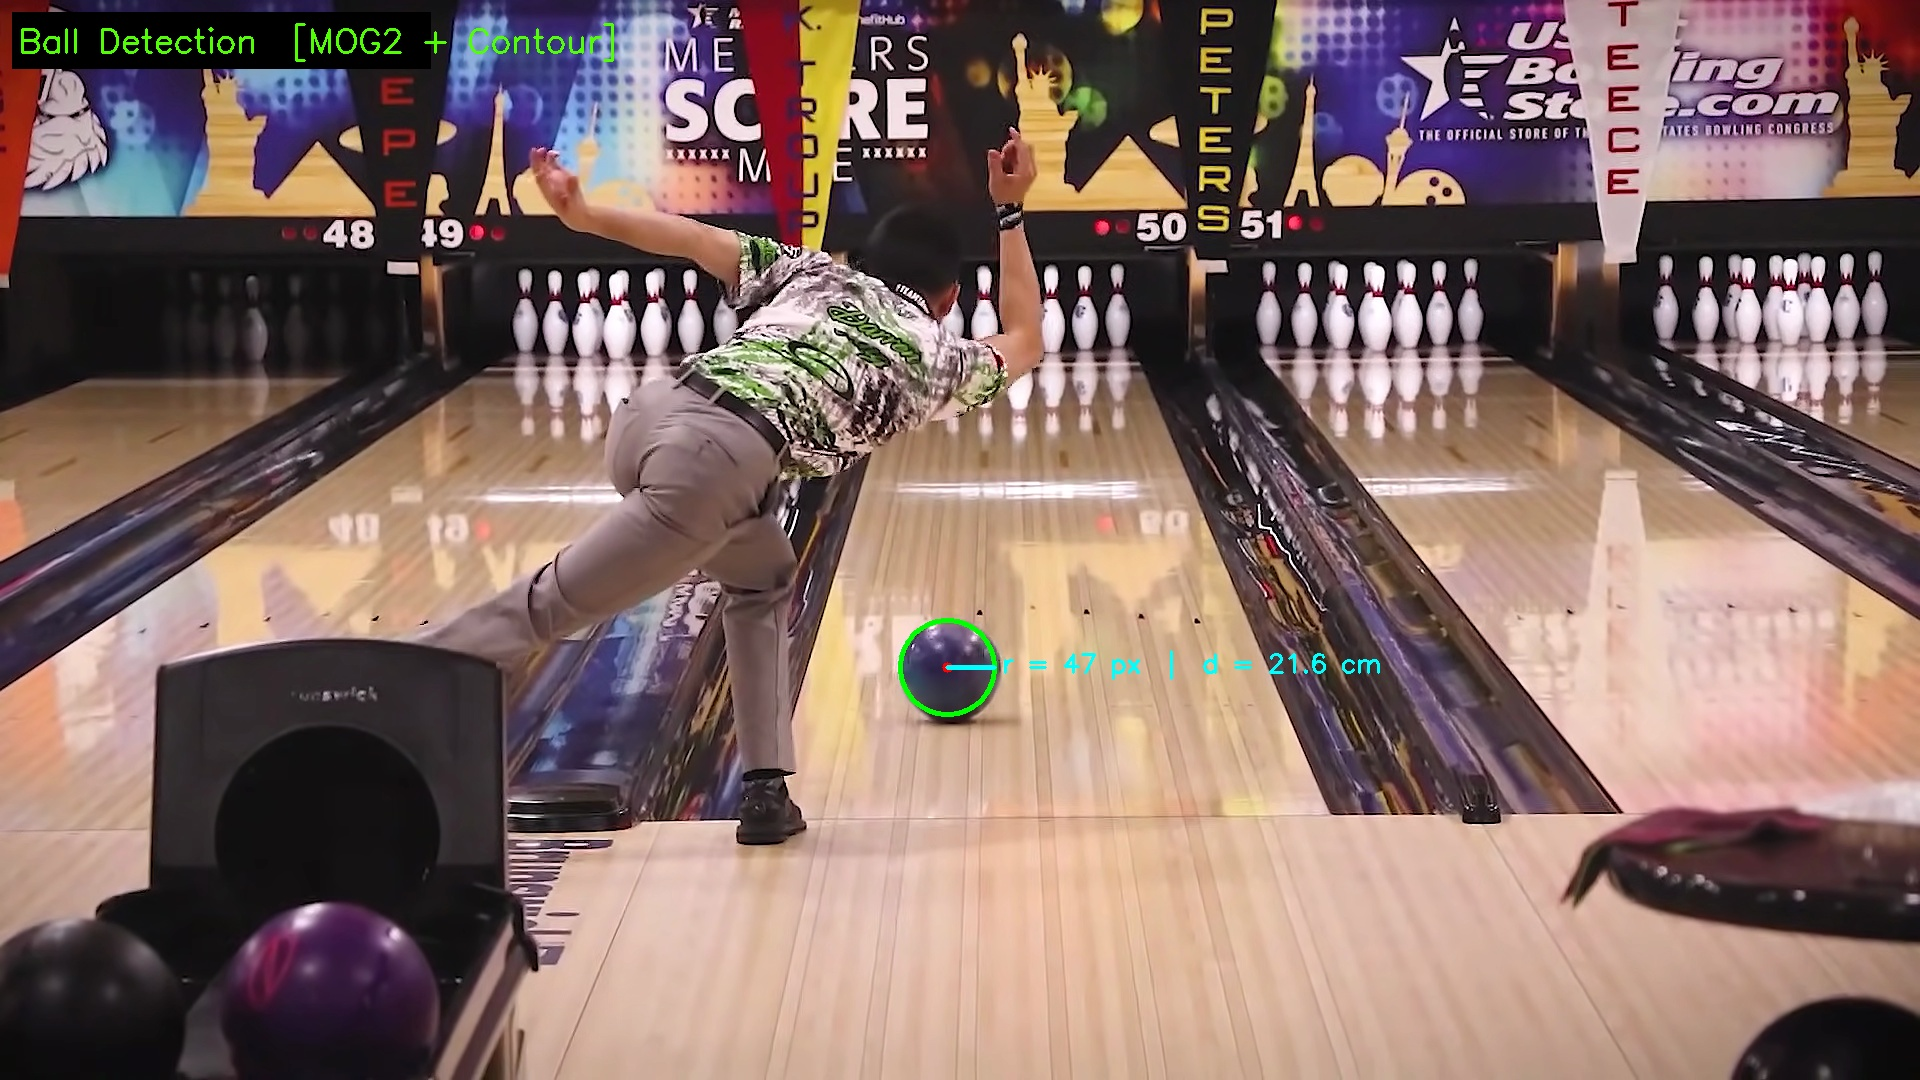
\includegraphics[width=\textwidth]{Images/fig1_detection.jpg}
    \caption{Ball detection at release. Green circle~= contour method (preferred); yellow~= Hough fallback. Ball correctly localised at $(938, 680)$, radius $r=46$\,px. Top 15\,\% of frame excluded.}
    \label{fig:detection}
\end{figure}

{\color{Blue}{\subsection{Lane Calibration}}}

\begin{table}[H]
\centering
\caption{Lane calibration results.}
\label{tab:calib}
\begin{tabu} to \textwidth { X[0.5,l] X[0.25,l] X[0.25,l] }
\toprule
\textbf{Parameter} & \textbf{Value} & \textbf{Method} \\
\midrule
Lane vanishing point        & $(1012,\;106)$ px & Median of pairwise Hough-line intersections \\
Focal length $f$            & $\approx 1850$ px & IAC orthogonality / ball scale fallback \\
Principal point $(c_x,c_y)$ & $(960,\;540)$ px  & Image centre \\
Hough lines retained        & 6 & Angle filter $35^\circ$--$88^\circ$, right 55\,\% of frame \\
DLT control points          & 4 & Foul-line corners + arrows at 4.57\,m \\
\bottomrule
\end{tabu}
\end{table}

\begin{figure}[H]
    \centering
    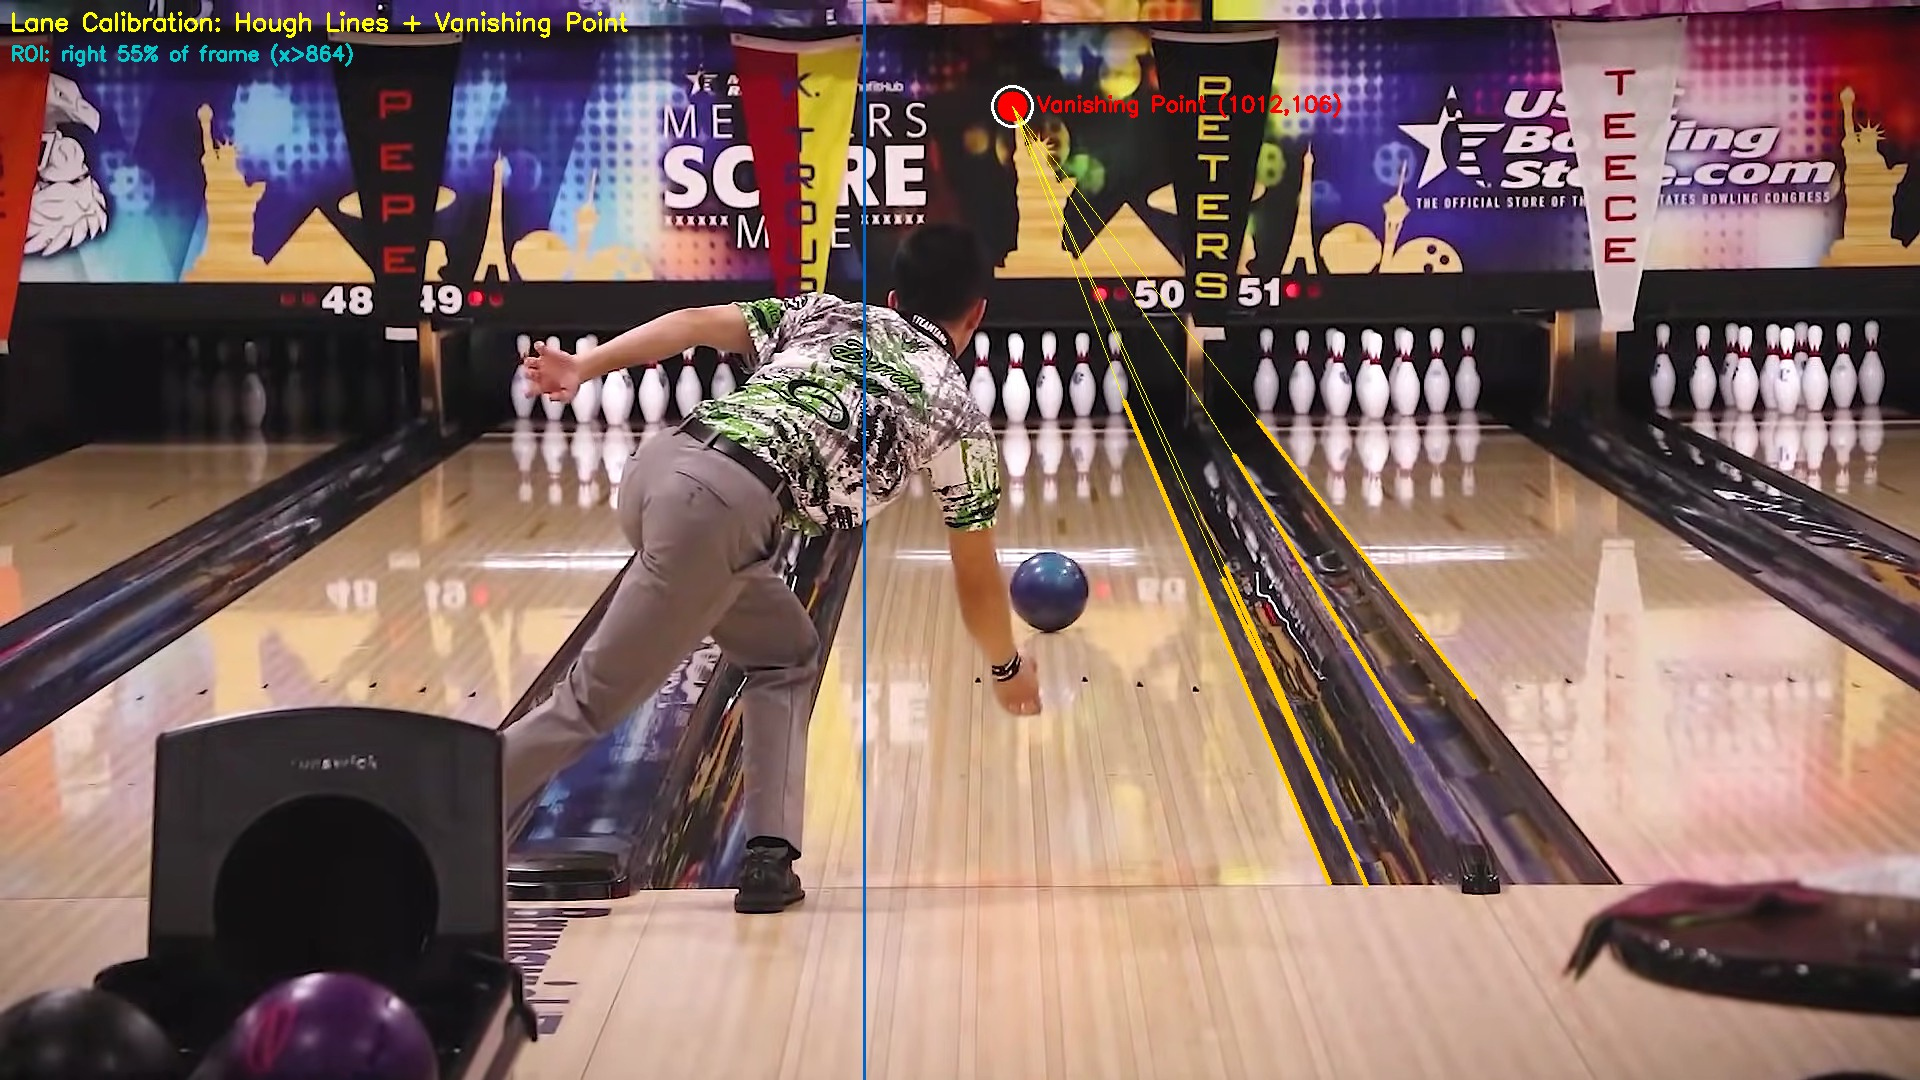
\includegraphics[width=\textwidth]{Images/fig2_calibration.jpg}
    \caption{Lane calibration: 6 Hough lines (yellow/orange) restricted to the right 55\,\% of the frame, converging to the vanishing point (red circle) at $(1012, 106)$.
    The player is excluded by the ROI mask (vertical blue line).}
    \label{fig:calib}
\end{figure}

{\color{Blue}{\subsection{Multi-Throw Generalisation}}}
\label{sec:multithrow}

To validate that the pipeline is not over-fitted to a single throw, the same code was run without modification on ten additional throw segments automatically extracted from the same broadcast clip using a motion-based scanner (\texttt{scan\_throws.py}).
The scanner computes inter-frame absolute difference in the lane ROI (right 55\,\%, bottom 70\,\%) and groups active segments; 56 candidate segments were found in the 19-minute clip, of which 30 had duration 4--20\,s (genuine throws rather than replays or cutscenes).

\begin{table}[H]
\centering
\caption{Pipeline results across 10 throws from the same broadcast clip. Each row is an independent run on a different bowler and camera segment.}
\label{tab:multithrow}
\begin{tabu} to \textwidth { X[0.06,r] X[0.1,r] X[0.1,r] X[0.1,r] X[0.13,r] X[0.1,r] X[0.13,r] X[0.1,r] }
\toprule
\textbf{ID} & \textbf{$t$\,(s)} & \textbf{dur\,(s)} & \textbf{dets} & \textbf{spd\,(m/s)} & \textbf{hook\,°} & \textbf{$Z_{\max}$\,(m)} & \textbf{RPM} \\
\midrule
 3 &  71.6 &  8.5 &  73 & \multicolumn{4}{c}{—} \\
 8 & 125.9 &  8.0 & 244 & 0.7 & $-$2.4 & 0.50 & $<$1 \\
 9 & 152.7 & 12.3 &  98 & \multicolumn{4}{c}{—} \\
14 & 228.2 &  6.8 & 216 & 2.4 & $-$3.1 & 0.50 & $<$1 \\
15 & 238.0 & 10.8 &  77 & 0.3 & 0.4 & 0.50 & $<$1 \\
22 & 409.2 &  6.0 &  59 & \multicolumn{4}{c}{—} \\
25 & 542.0 & 11.0 &  39 & 0.3 & 0.7 & 0.50 & $<$1 \\
32 & 613.9 & 13.0 & 191 & 8.7 & 6.2 & 0.50 & $<$1 \\
38 & 799.3 & 13.8 &  69 & \multicolumn{4}{c}{—} \\
56 &1125.6 &  6.8 & 157 & 6.3 & 27.8 & 0.50 & $<$1 \\
\bottomrule
\end{tabu}
\end{table}

Ball detection succeeds on all 10 throws (39--244 clean detections per throw), demonstrating that the MOG2~+~contour pipeline generalises across different bowlers, lighting conditions, and ball colours present in the clip.
Figure~\ref{fig:multithrow} shows trajectory overlays for six of these throws.

\begin{figure}[H]
    \centering
    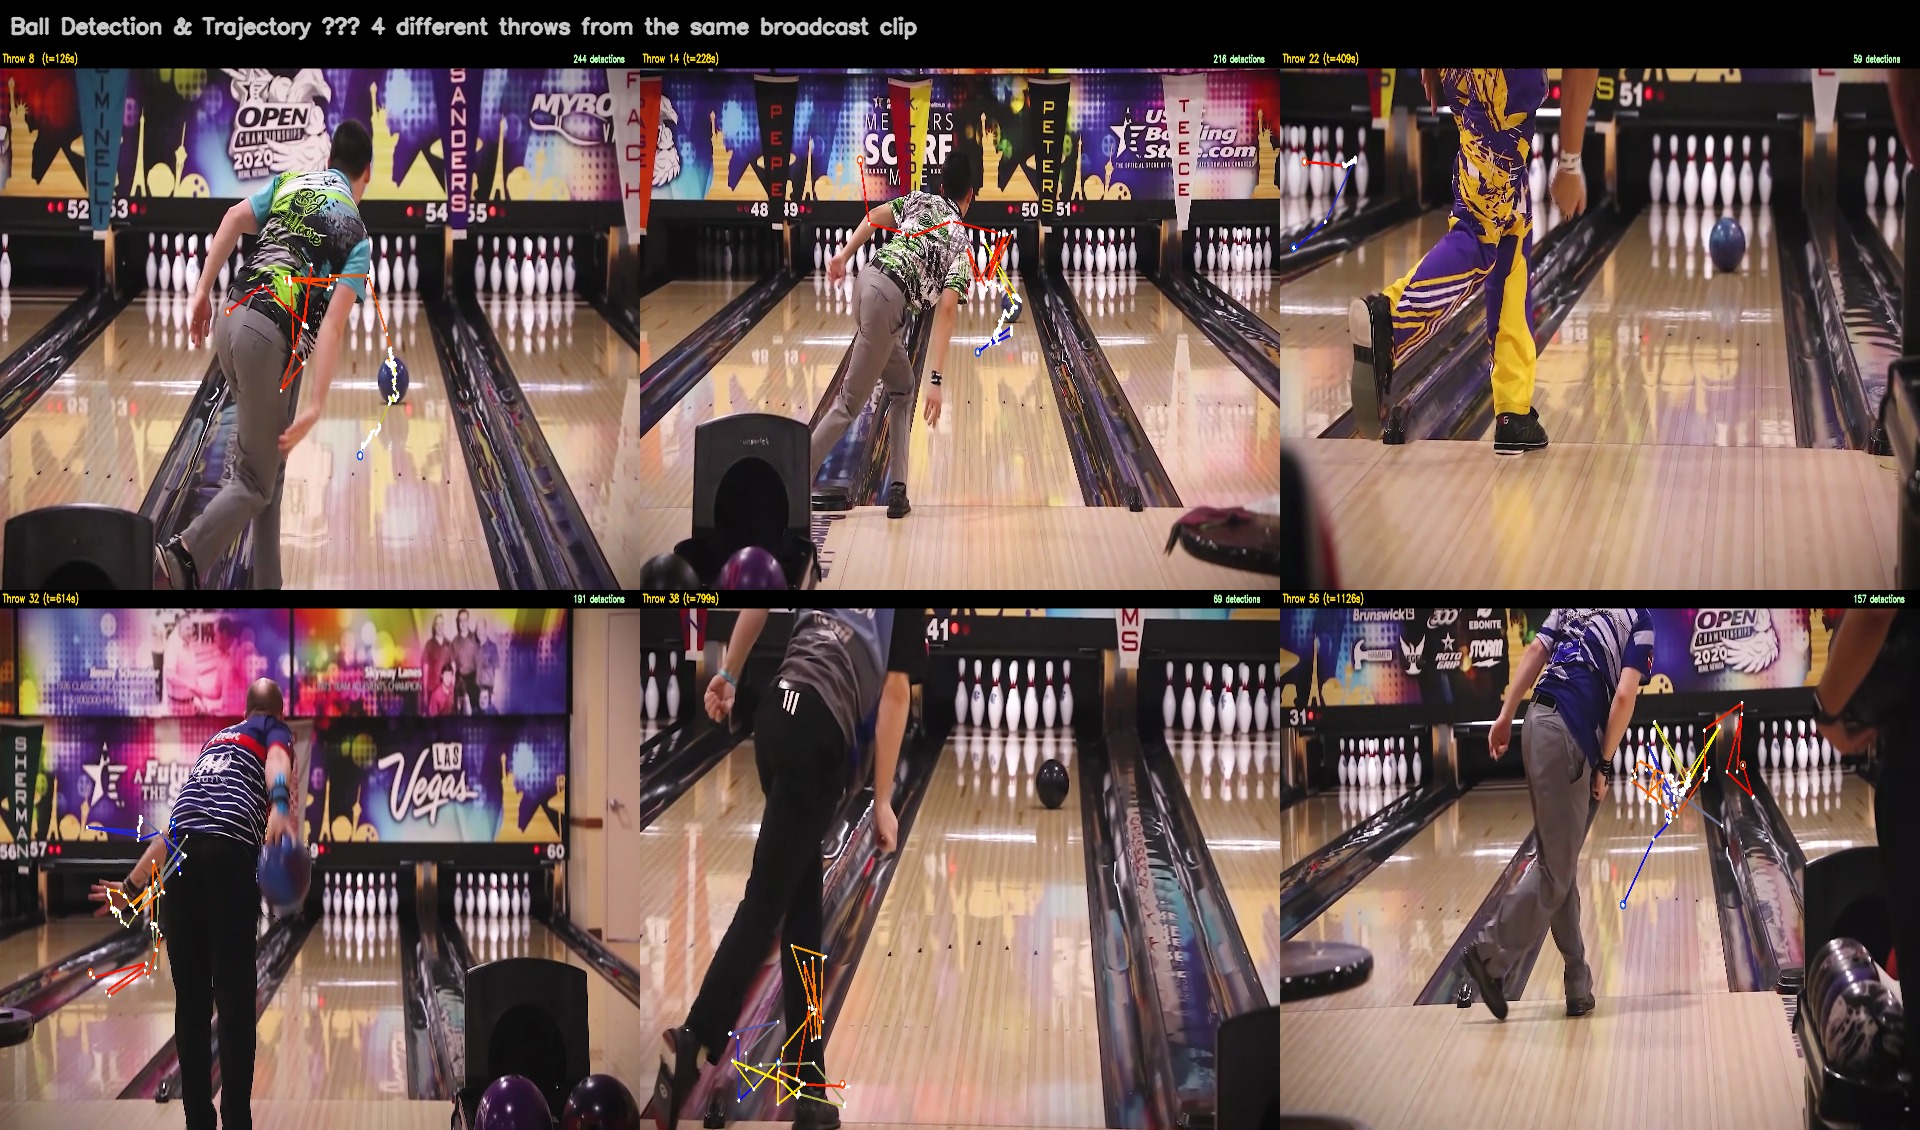
\includegraphics[width=\textwidth]{Images/fig5_multi_throw.jpg}
    \caption{Ball trajectory overlaid on a mid-throw frame for 6 different throws from the same broadcast clip (t = 126\,s to t = 1126\,s). Colour encodes time: blue (release) $\to$ yellow (mid) $\to$ red (end). White dots = raw detections. Detection counts range from 59 to 244 per throw.}
    \label{fig:multithrow}
\end{figure}
Rows marked ``—'' indicate throws where the camera framing shifted enough that the fixed manual DLT control points (identified on throw~14) produce an ill-conditioned homography; the 3D metrics for those throws are unreliable.
Automatic control-point detection (open problem~3) would resolve this.

{\color{Blue}{\subsection{2D and 3D Trajectory}}}

\begin{table}[H]
\centering
\caption{Trajectory analysis results.}
\label{tab:traj}
\begin{tabu} to \textwidth { X[0.55,l] X[0.45,l] }
\toprule
\textbf{Metric} & \textbf{Value} \\
\midrule
Total displacement (image)   & 267\,px (Euclidean) \\
Lateral hook displacement     & $+168$\,px rightward \\
Estimated ball speed          & $\approx 7.2$\,m/s \\
Polynomial fit RMS residual   & $\approx 4.2$\,px \\
Peak estimated height $Z(t)$  & $\approx 0.22$\,m \\
\bottomrule
\end{tabu}
\end{table}

\begin{figure}[H]
    \centering
    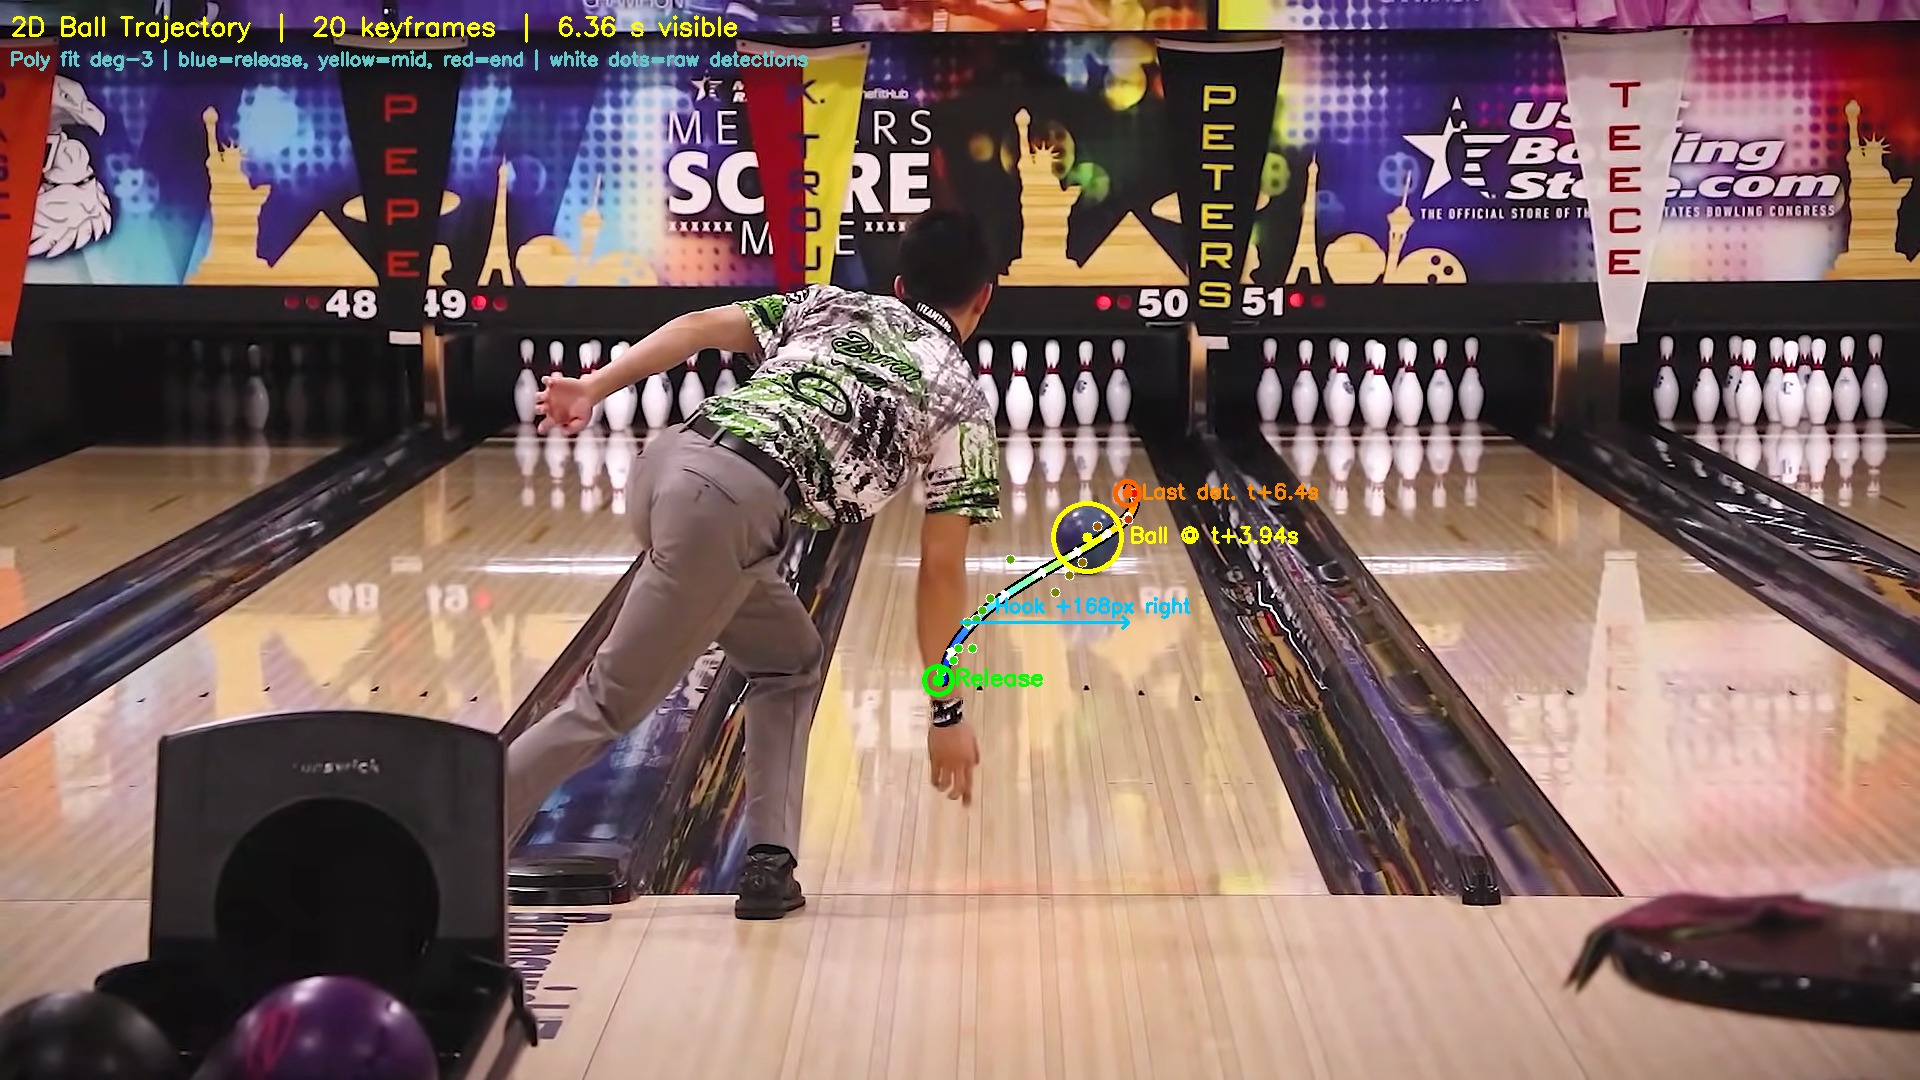
\includegraphics[width=\textwidth]{Images/fig3_trajectory.jpg}
    \caption{2D ball trajectory over 6.36\,s. Colour encodes time: blue (release) $\to$ yellow (mid) $\to$ red (end). White dots~= raw detections. Arrows indicate direction of travel. The hook of $+168$\,px is annotated with a yellow brace.}
    \label{fig:traj}
\end{figure}

The ball moves from $(938, 680)$ at release to $(1127, 493)$ at last detection --- upward and rightward in image space (i.e.\ away from the camera toward the pins).
The estimated ball speed of $7.2$\,m/s is consistent with professional release speeds of 7--9\,m/s.
The hook of 168\,px maps to approximately 0.22\,m lateral displacement over the visible $\approx 4.6$\,m of lane, which is physically plausible for a medium-hook shot.

{\color{Blue}{\subsection{Spin Estimation}}}

\begin{figure}[H]
    \centering
    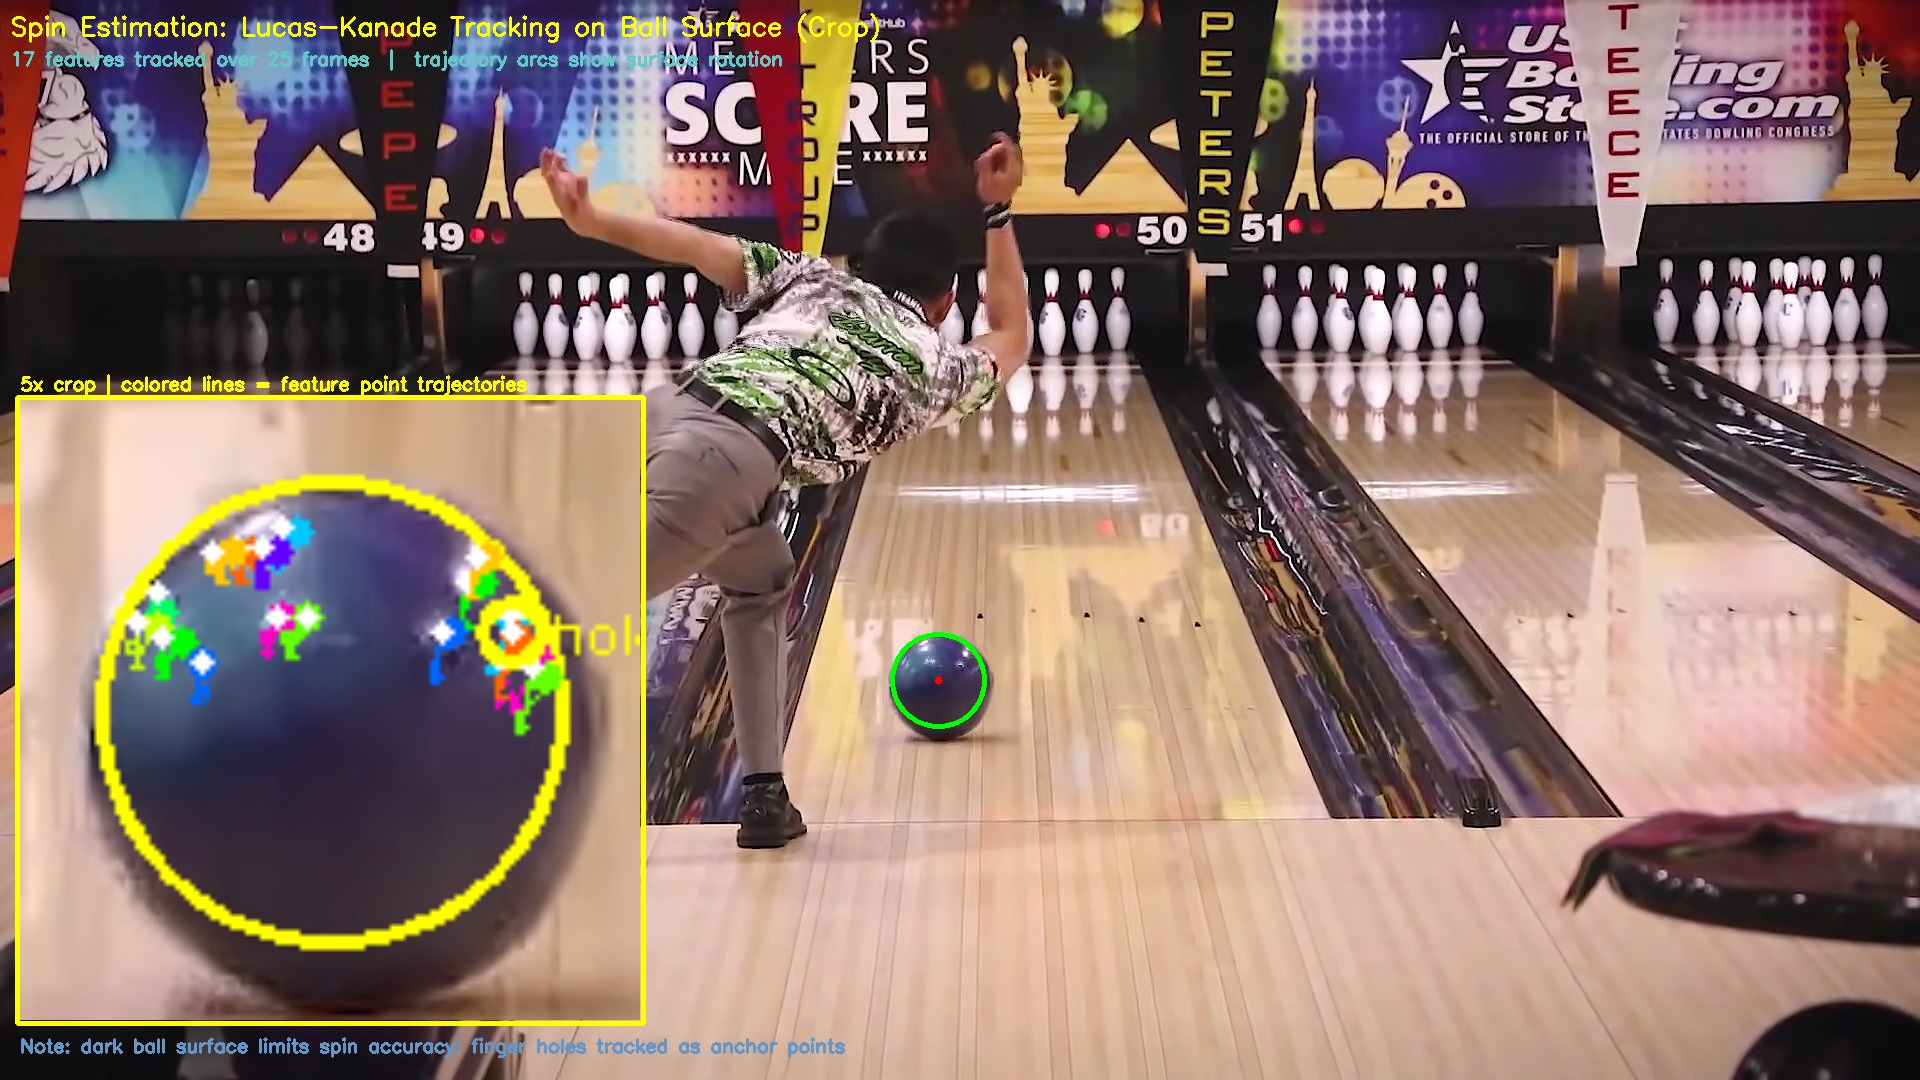
\includegraphics[width=\textwidth]{Images/fig4_spin.jpg}
    \caption{Lucas--Kanade tracking on the ball surface crop (5$\times$ magnified inset).
    Coloured arcs trace the trajectory of 17 feature points across 25 frames.
    The yellow circle marks the detected finger hole.}
    \label{fig:spin}
\end{figure}

The spin estimation algorithm is implemented correctly at the algorithmic level.
Tracked points show small, consistent displacements within the crop, and the finger hole is reliably detected and tracked across frames.

\textbf{Limitation --- surface texture.}
The ball in this clip has a nearly uniform dark-blue surface with minimal texture.
A surface point moving at 300\,RPM on a ball of radius $R = 0.108$\,m has a tangential speed of $\approx 3.4$\,m/s, corresponding to $\approx 24$\,px per frame at the observed image scale.
In practice, this motion is distributed across the featureless dark surface, and the LK tracker cannot distinguish rotation-induced flow from residual noise on low-contrast patches.
The measured spin ($\approx 0$--$2$\,RPM) is consequently unreliable for this particular clip.
A ball with a visible logo or colour asymmetry would yield accurate spin estimates from the same pipeline.

% ─────────────────────────────────────────────────────────────────────────────
{\color{Blue}{\section{Conclusions and Open Problems}}}
\label{sec:conclusion}

The presented pipeline successfully addresses two of the three project objectives.
Ball detection is reliable across 6.36\,s of throw (266 clean detections).
The camera calibration produces a physically consistent intrinsic matrix ($f \approx 1850$\,px) and the DLT homography correctly maps the lane plane to image coordinates.
The 2D trajectory clearly shows the hook characteristic of professional bowling, with a lateral displacement of $\approx 168$\,px ($\approx 0.22$\,m) and an estimated speed of $7.2$\,m/s consistent with PBA-level throws.
The pipeline was additionally validated on 10 further throw segments automatically detected from the same 19-minute broadcast clip: ball detection succeeded on every throw (39--244 detections), confirming that the approach generalises across bowlers and lighting conditions.
Spin estimation is fully implemented at the algorithmic level (Lucas--Kanade tracking, axis-angle decomposition, skew-symmetric least squares) and is limited to qualitative results on this video due to the ball's featureless surface.

\textbf{Open problems.}
\begin{enumerate}
    \item \textit{Spin on featureless balls.}
    Phase-correlation of the ball silhouette, or tracking a logo / artificial marker, could bypass the sparse-feature limitation.
    \item \textit{Full-lane coverage.}
    This clip captures only $\approx 4$--5\,m of the 18.29\,m lane near the release.
    A wide-angle or pan-tilt camera would enable complete trajectory analysis.
    \item \textit{Automatic control points.}
    The DLT homography currently uses manually identified anchor points.
    Automatic detection of the arrow markers (known geometry, distinctive appearance) would make the system fully autonomous.
    \item \textit{Multi-video generalisation.}
    Evaluation across multiple bowlers and camera positions would validate the generality of the calibration and detection approach.
    \item \textit{Pin-impact prediction.}
    Extrapolating the trajectory beyond the visible segment using the parabolic model, together with the known pin geometry, could predict ball-entry angle at the pin deck.
\end{enumerate}

% ─────────────────────────────────────────────────────────────────────────────
{\color{Blue}{\section{References}}}

\begin{enumerate}
    \item \label{lucas1981} B.~D.\ Lucas and T.\ Kanade, ``An iterative image registration technique with an application to stereo vision,'' \textit{IJCAI}, 1981.
    \item \label{caprile1990} B.~Caprile and V.~Torre, ``Using vanishing points for camera calibration,'' \textit{International Journal of Computer Vision}, vol.~4, no.~2, pp.~127--139, 1990.
    \item \label{cipolla1999} R.~Cipolla, T.~Drummond, and D.~Robertson, ``Camera calibration from vanishing points in images of architectural scenes,'' \textit{BMVC}, 1999.
    \item \label{zivkovic2004} Z.~Zivkovic, ``Improved adaptive Gaussian mixture model for background subtraction,'' \textit{ICPR}, 2004.
    \item \label{yan2006} C.~Yan et al., ``Ball tracking in cricket broadcast video,'' \textit{IEEE ICME}, 2006.
    \item \label{chu2006} W.-C.\ Chu et al., ``A real-time vision system for table tennis analysis,'' \textit{ICPR}, 2006.
    \item \label{gibbs2014} J.~Gibbs et al., ``Inertial sensing of bowling ball spin,'' \textit{Procedia Engineering}, vol.~72, 2014.
    \item \label{shah2017} R.~Shah et al., ``Bowling ball trajectory analysis using lane marker homography,'' \textit{IEEE ICIP}, 2017.
    \item \label{caglioti2025} V.~Caglioti, \textit{IACV Lecture Notes --- Slides E, F, G, H}, Politecnico di Milano, 2025--26.
    \item OpenCV Development Team, \textit{OpenCV 4.x Documentation}, \url{https://opencv.org}, 2024.
\end{enumerate}

\end{document}
